% ============================================================
% 第三章 充气伞形结构设计
% ============================================================

\chapter{充气伞形结构设计}

\section{充气结构力学基础}

\subsection{薄壁充气结构受力原理}
充气结构（Pneumatic Inflatable Structure）是一类依靠内部气体压力维持形态与结构刚度的柔性结构体系。
其基本工作原理可通过薄壁压力容器理论加以描述：当气囊内部气体压力 $p$ 大于外部大气压时，
气囊壁面承受周向（环向）拉应力与轴向拉应力，在两者的共同作用下气囊维持充气形态并具备抵抗外力变形的能力。
对于简化为圆柱形薄壁气囊的情形，气囊壁面所受环向应力 $\sigma_\theta$ 与轴向应力 $\sigma_z$ 分别为：
\begin{equation}
    \sigma_\theta = \frac{p \cdot r}{t}
    \label{eq:hoop_stress}
\end{equation}
\begin{equation}
    \sigma_z = \frac{p \cdot r}{2t}
    \label{eq:axial_stress}
\end{equation}
其中 $p$ 为充气表压（Pa），$r$ 为气囊内半径（m），$t$ 为气囊壁厚（m）。
由此可见，环向应力是轴向应力的两倍，气囊最容易沿轴向方向开裂，
这也是气囊材料选型中需要重点考量环向强度的原因。

\subsection{充气压力与结构刚度的关系}
充气结构的等效抗弯刚度随充气压力的增大而提高。
在小变形假设下，充气圆柱梁在承受外部横向载荷（如飞行器的结构重力与旋翼推力）时，其内部受力状态与弯曲变形特征如图~\ref{fig:inflatable_bending}所示\cite{Sun2024}。

\begin{figure}[htbp]
    \centering
    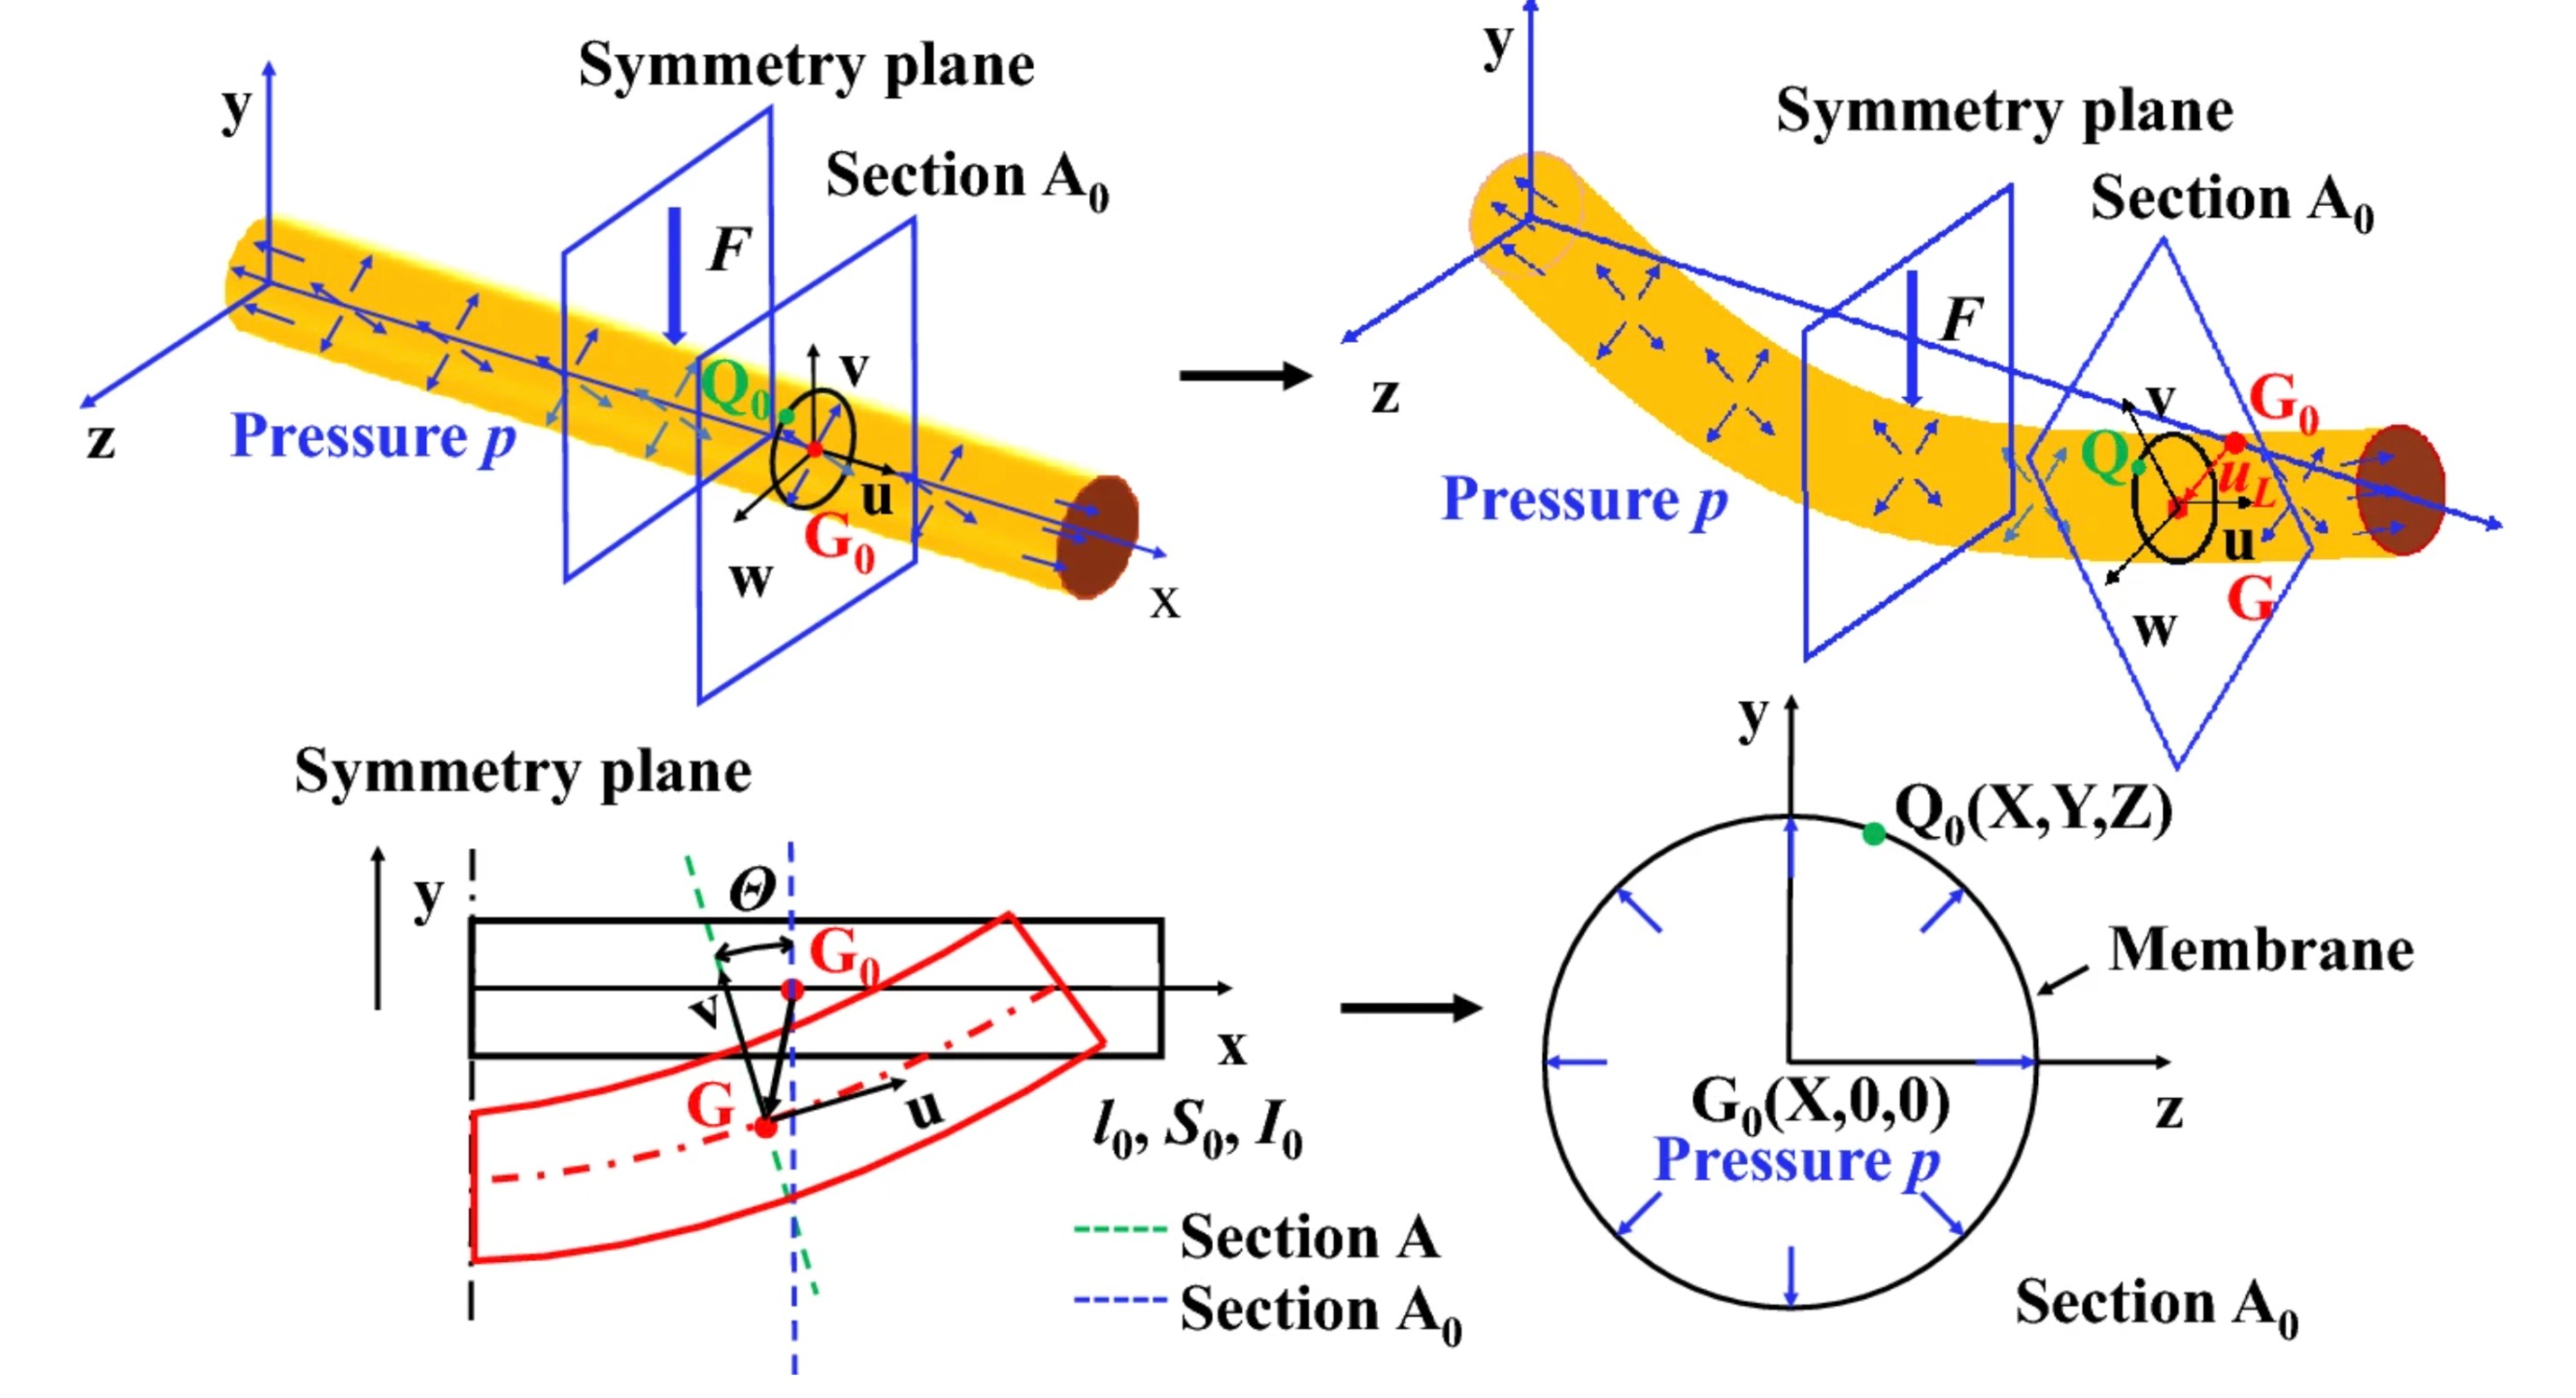
\includegraphics[width=0.85\textwidth]{figures/fig3_1_inflatable_bending.pdf}
    \caption{圆柱形充气梁弯曲受力模型与截面变形示意图（图片来源：Sun 等, 2024~\cite{Sun2024}）}
    \label{fig:inflatable_bending}
\end{figure}

如图~\ref{fig:inflatable_bending}右下角的截面图所示，内部气体压力 $p$ 均匀作用于气囊内壁，使膜材处于预张紧状态。
充气压力越高，气囊壁面初始张力越大，结构对横向弯曲载荷的抵抗能力越强；
当充气压力不足时，气囊将在弯曲载荷下出现局部塌陷，失去承载能力。
近年来，Sun 等人的研究进一步表明，充气梁在弯曲过程中的剪切效应高度依赖于截面特征，且内压的变化会显著改变充气梁的几何参数与动态刚度\cite{Sun2024}。
这一特性决定了充气结构在使用过程中需要维持一定的最低工作气压，以保证结构刚度满足飞行载荷要求。

本文所采用的充气气柱为市售标准快递气柱，如图~\ref{fig:aircolumn_compare}所示，其充气后圆柱直径约为 $1.7\sim2.0$\,cm，
充气工作气压约为 $0.05\sim0.1$\,MPa（表压）。
气柱材料为PA（尼龙）复合薄膜，具有良好的气密性、一定的柔韧性以及对水汽的阻隔能力，
能够应对户外雨天使用场景。

% ----------------------------------------------------------
% [图片占位 Fig.3.2] ★需要拍摄★
% 内容：气柱实物对比照片
%   左：排气折叠状态（扁平薄膜状）
%   右：充气后圆柱状态，旁边放尺子标注直径约1.9cm
%   用手机拍摄即可，光线均匀，白色背景最佳
\begin{figure}[htbp]
    \centering
    \includegraphics[width=0.65\textwidth]{figures/fig3_2_aircolumn_compare.pdf}
    \caption{快递气柱排气状态（左）与充气状态（右）对比}
    \label{fig:aircolumn_compare}
\end{figure}

% ----------------------------------------------------------



\section{充气伞形骨架结构设计}

\subsection{结构概念与设计思路}

飞行雨伞的充气骨架系统承担两项核心功能：其一，作为多旋翼飞行器的机体骨架，
为四组旋翼动力单元提供安装位置和结构支撑；其二，作为伞面的支撑框架，
维持TPU伞面的展开形态，实现有效的遮雨遮阳防护。
骨架系统的整体三维结构如图~\ref{fig:cad_overview}所示。

\begin{figure}[htbp]
    \centering
    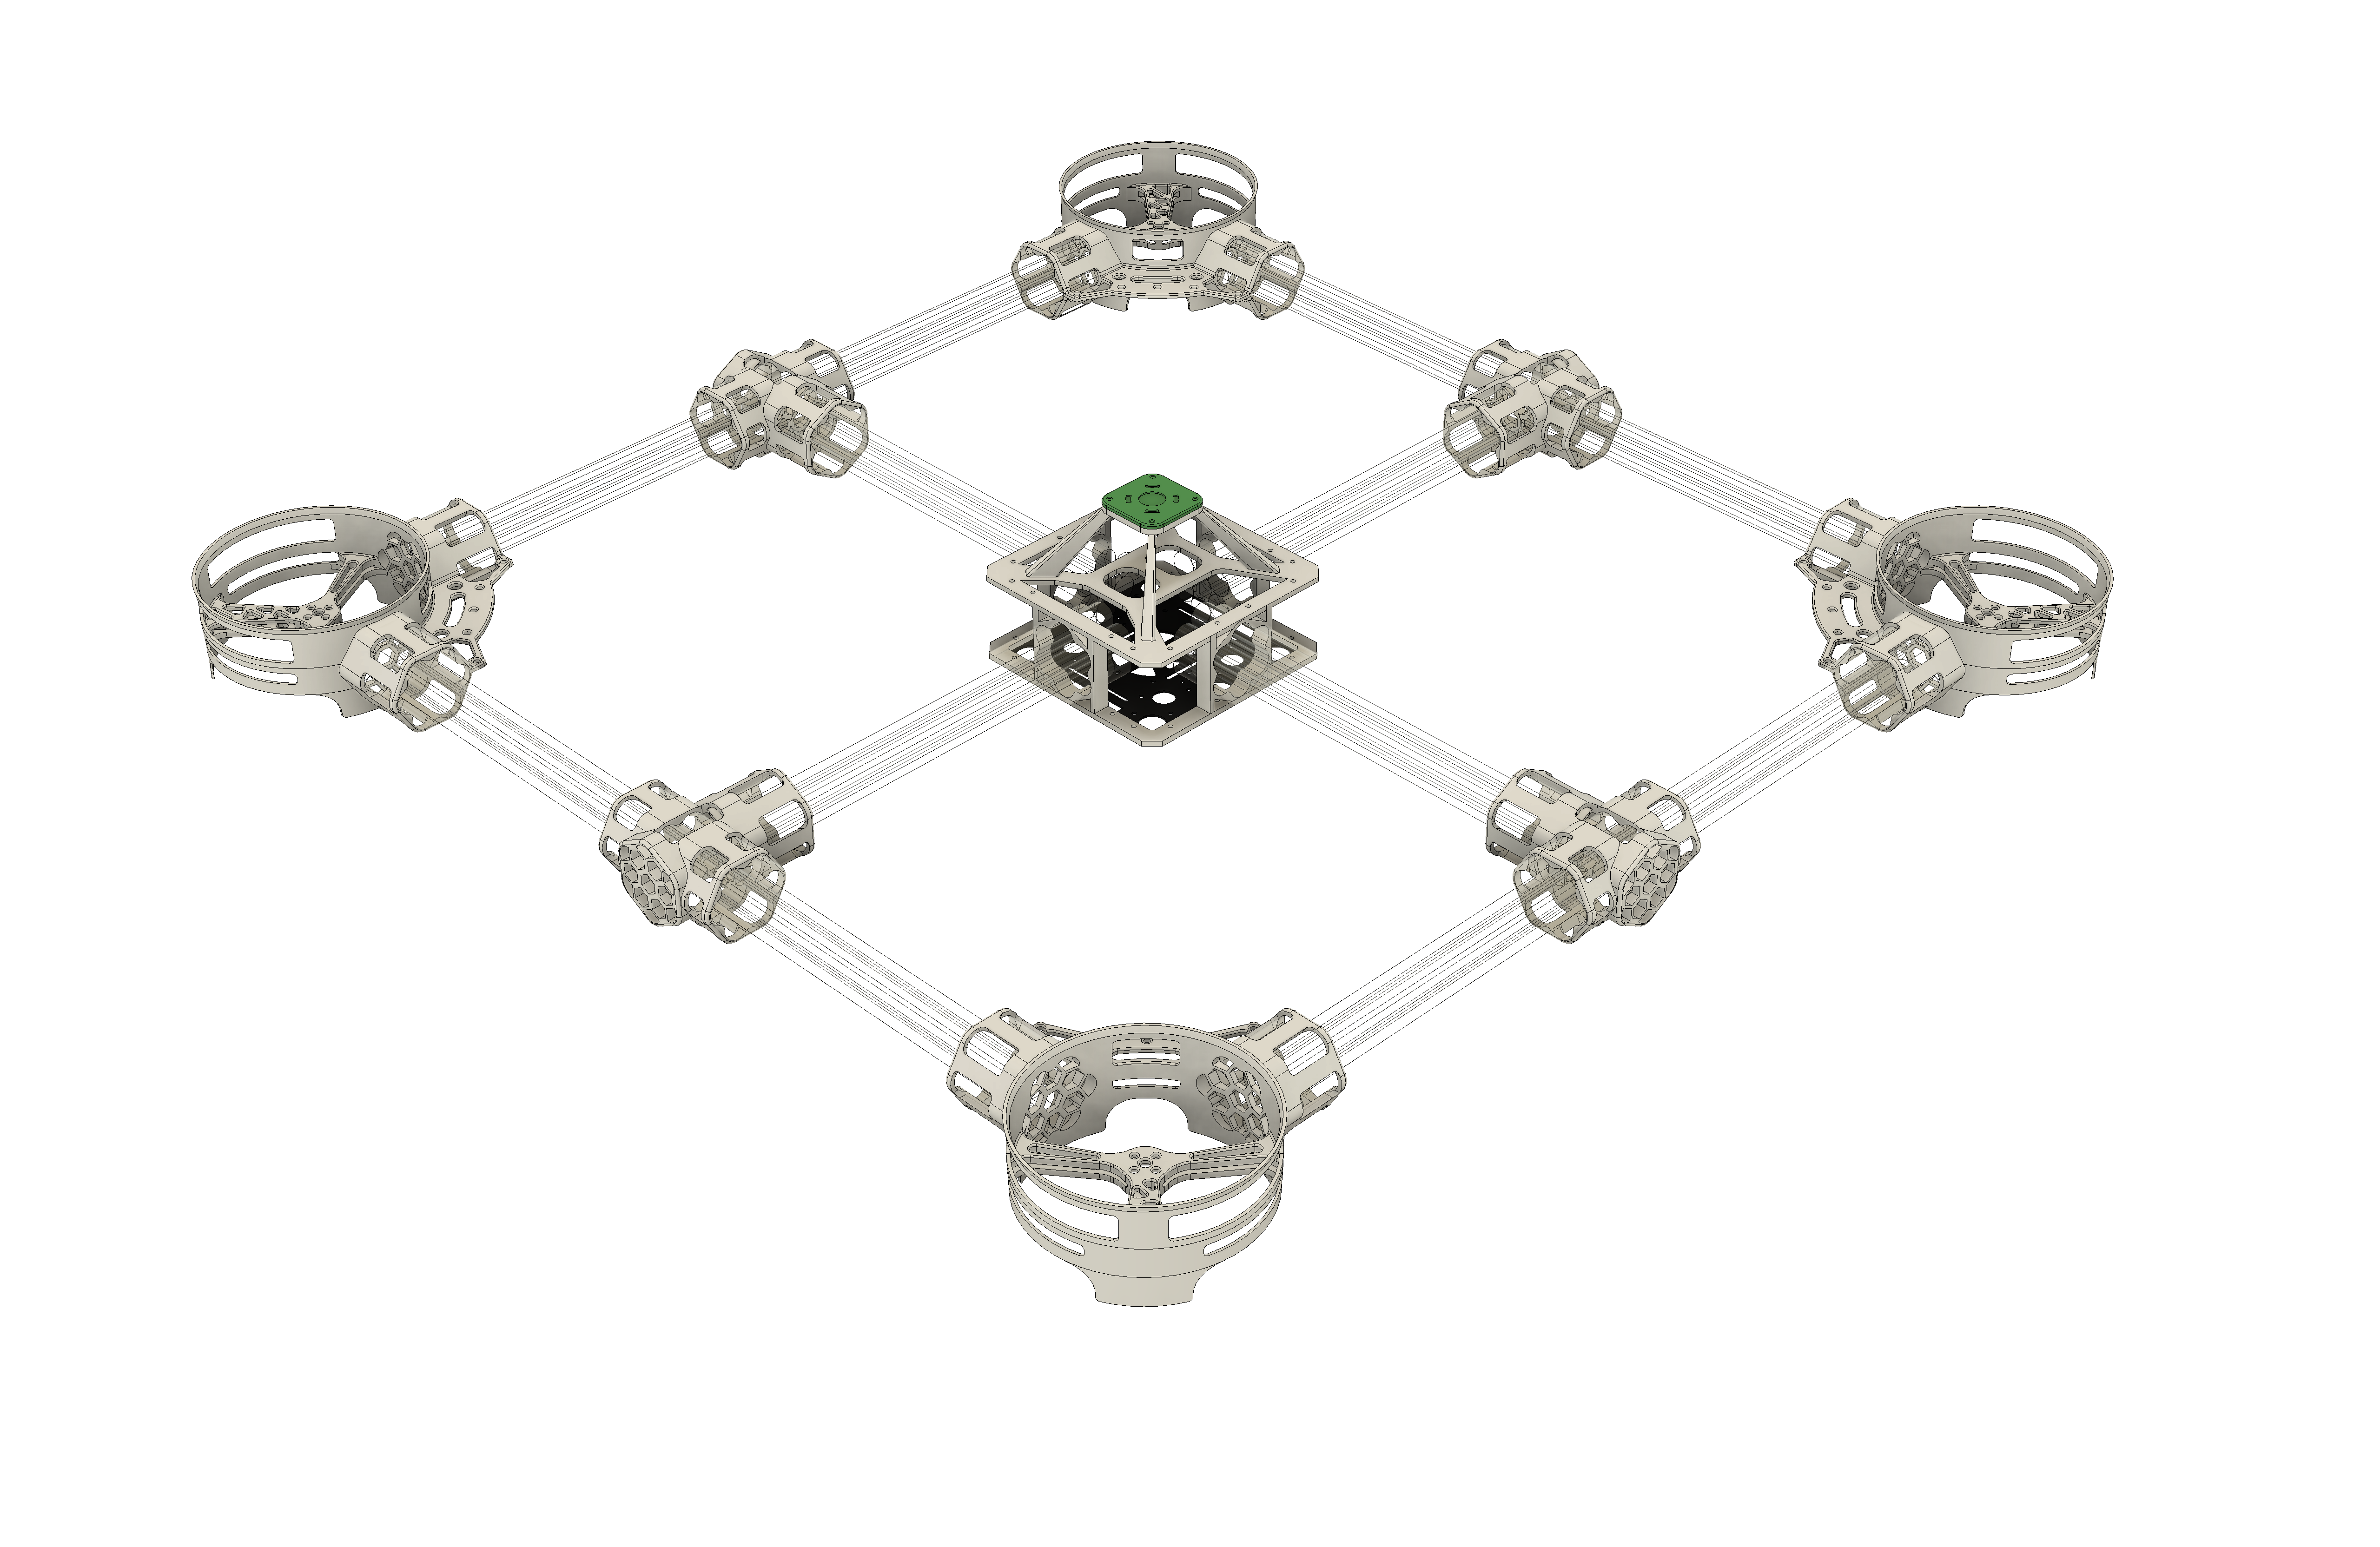
\includegraphics[width=0.80\textwidth]{figures/fig3_1_cad_overview.png}
    \caption{充气伞形骨架系统整体三维结构（Fusion 360）}
    \label{fig:cad_overview}
\end{figure}

本系统采用\textbf{气柱-节点模块化骨架}设计思路：以标准快递气柱作为承力杆件，
以 PLA（聚乳酸）3D 打印节点作为连接与固定元件，构成正方形平面桁架式骨架结构。
气柱在排气状态下可完全压缩折叠，体积接近零；充气后具备一定的结构刚度，
能够承受旋翼推力产生的局部集中载荷。
系统中\textbf{不使用任何刚性碳纤维或金属结构件}，气柱本身即是机臂上的唯一承力构件，
"充气即成形、排气即收纳"的形态切换由此得以实现。

\subsection{骨架几何构型}

骨架采用正方形平面布局，四角各安装一套旋翼动力单元（含电机、电调与3D打印旋翼保护架）。
各旋翼单元通过气柱与相邻节点连接件对接，形成闭合的正方形框架，
如图~\ref{fig:frame_cad}所示。骨架的主要几何参数如表~\ref{tab:frame_dimensions}所示。

\begin{table}[htbp]
    \centering
    \caption{骨架主要几何参数}
    \label{tab:frame_dimensions}
    \begin{tabular}{llll}
        \toprule
        参数             & 设计值    & 实测值       & 说明 \\
        \midrule
        骨架外框边长      & 888\,mm  & 870\,mm     & 气柱充气后自然收缩 \\
        对角旋翼轴距      & 1256\,mm & 1230\,mm    & 对角线尺寸 \\
        单边气柱标称长度   & 600\,mm  & 560\,mm     & 充气后收缩约7\% \\
        单气柱充气直径    & 约20\,mm & 17$\sim$20\,mm & 标准快递气柱 \\
        旋翼保护架外径    & 146\,mm  & 146\,mm     & 3D打印PLA \\
        \bottomrule
    \end{tabular}
\end{table}

设计值与实测值存在约2\%的尺寸偏差，主要来源于气柱充气后的轴向收缩效应
以及节点接口处气柱端部薄膜堆积。在工程应用中，以实测值作为结构性能分析的基准参数。

% ----------------------------------------------------------
% [图片占位 Fig.3.3] ★可直接使用已有截图★
% 内容：骨架CAD设计俯视图（带尺寸标注）
%   即之前发给我的"888.866mm"测量截图
%   建议：在CAD中再额外标注对角线1256mm和保护圈直径146mm后截图
%   裁去右侧属性面板，只保留模型区域
\begin{figure}[htbp]
    \centering
    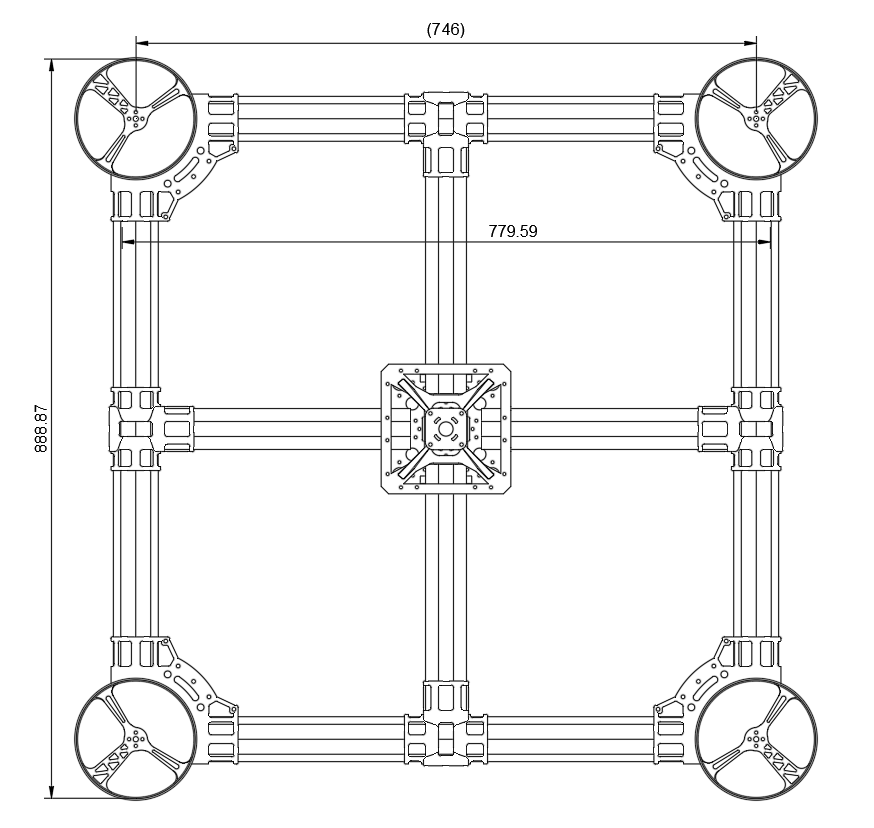
\includegraphics[width=0.75\textwidth]{figures/fig3_3_frame_cad.png}
    \caption{飞行雨伞骨架CAD设计俯视图}
    \label{fig:frame_cad}
\end{figure}
% ----------------------------------------------------------

\subsection{气柱布置方案与连接设计}
每条骨架边由七根标准快递气柱单元卷绕组合而成，气柱两端通过PLA节点连接件固定。
七根气柱按蜂窝式排列——中心1根、外围6根紧密围绕——充气后各气柱单元相互挤压，
自然形成近似正六边形的组合截面，等效外径约为 54.2\,mm。
这种多气柱并联组合方案在单个气柱单元发生漏气时，
其余气柱仍可维持骨架基本形态，具备一定的冗余容错能力。

节点连接件同时承担以下功能：气柱端口密封固定、相邻两边骨架的正交对接、
旋翼安装座集成（四角节点），以及中心飞控安装平台的连接接口。

为确保柔性气柱束与刚性PLA节点之间的连接强度，本系统设计了与七根气柱卷绕截面相匹配的
专用孔道结构。如图~\ref{fig:node_section}所示，节点连接件的内孔截面设计为
由三个半径 $R=10$\,mm 的外凸圆弧与半径 $R=5$\,mm 的内凹圆弧交替构成的三叶形轮廓，
相邻凸起间夹角为 120°。
三叶形的三个凸起分别对应七根气柱蜂窝截面外围的三对气柱，
孔道轮廓与气柱束充气后的自然膨胀形态高度吻合，形成有效的几何限位。
在实际装配中（如图~\ref{fig:node_assembly_real}所示），
气柱束穿过三叶形孔道后，在孔壁接触面处注入热熔胶进行二次固定，
冷却固化后同时起到增强轴向抗拉强度与辅助密封的作用。

\begin{figure}[htbp]
    \centering
    \begin{minipage}[b]{0.48\textwidth}
        \centering
        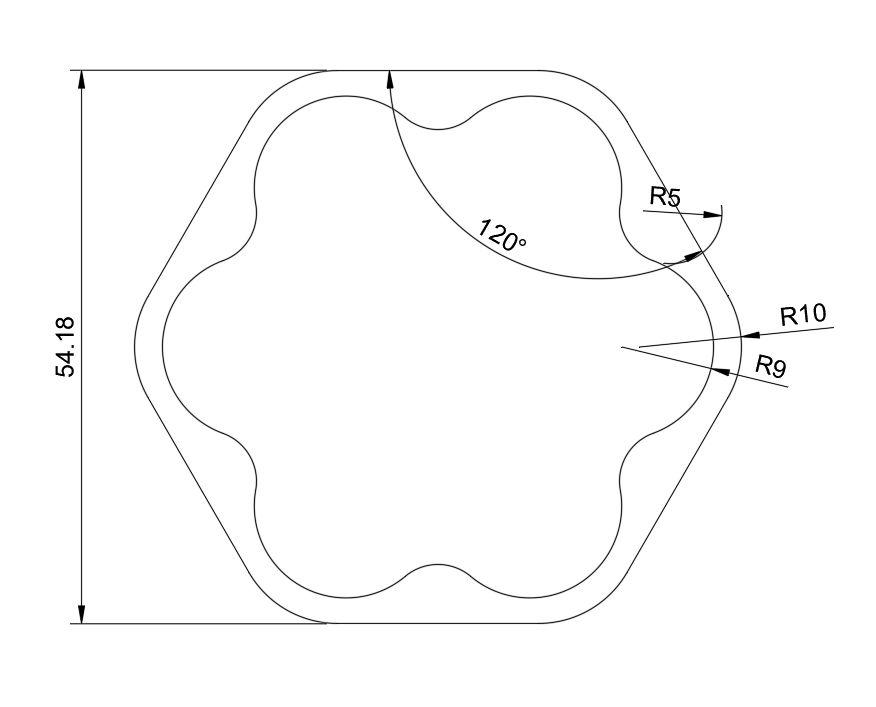
\includegraphics[width=\textwidth]{figures/fig3_node_section_cad.png}
        \caption{节点连接件截面CAD设计图}
        \label{fig:node_section}
    \end{minipage}
    \hfill
    \begin{minipage}[b]{0.48\textwidth}
        \centering
        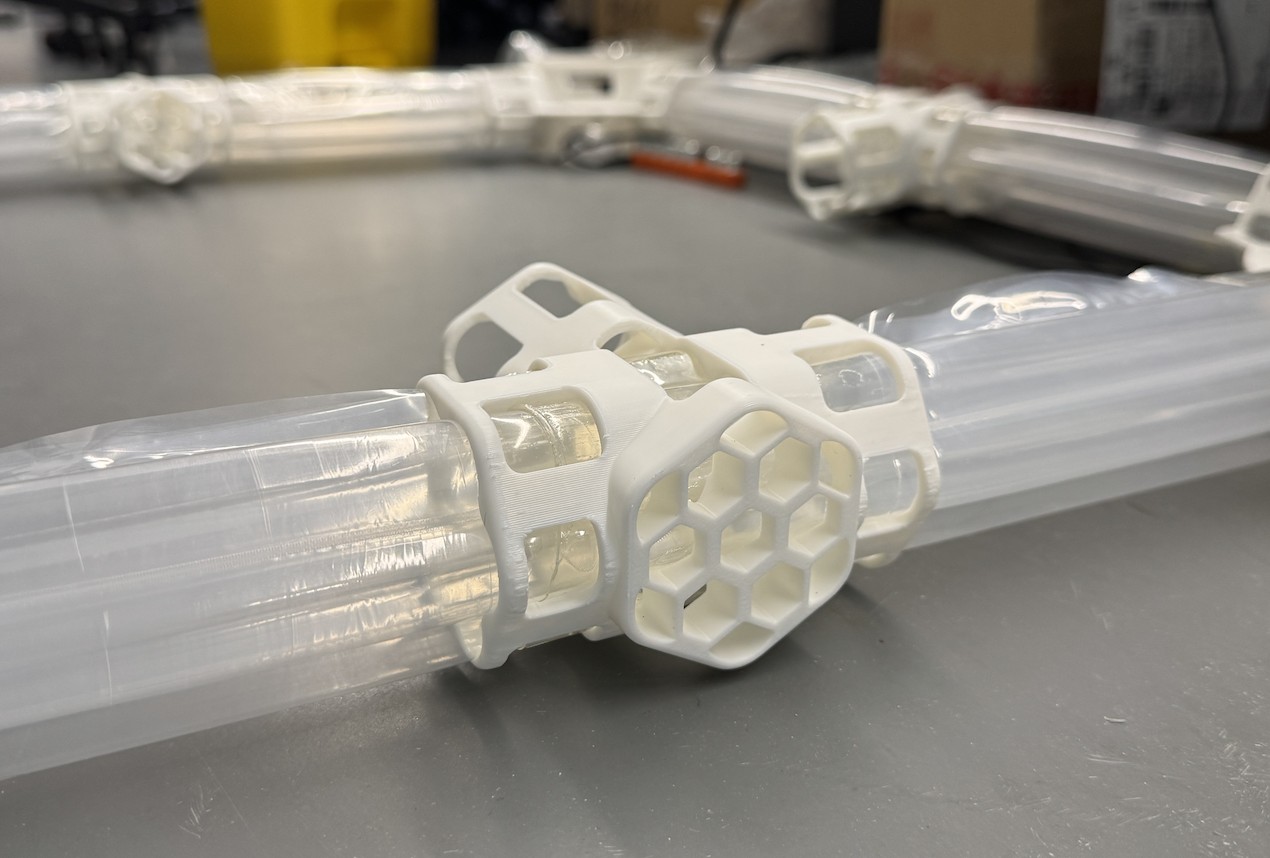
\includegraphics[width=\textwidth]{figures/fig3_node_assembly_real.png}
        \caption{气柱与PLA节点连接件实物装配图}
        \label{fig:node_assembly_real}
    \end{minipage}
\end{figure}

在实际装配中（如图~\ref{fig:node_assembly_real}所示），
气柱穿过PLA连接件的孔道，孔道的几何形状对气柱形成了有效的物理限位，
防止气柱在受力时发生径向滑脱或扭转。
同时，在气柱与PLA孔壁的接触面之间注入热熔胶进行二次固定。
热熔胶冷却固化后，不仅增强了连接的轴向抗拉强度，还起到了进一步的密封作用。
全部PLA节点结构件由FDM工艺3D打印制作，材料为PLA。
这种多气柱并联设计在单个气囊发生漏气时，其余气柱仍可维持骨架基本形态，具备一定的冗余容错能力。

\subsection{骨架尺寸参数验证}
骨架的详细尺寸参数通过CAD装配模型进行了精确验证。
图~\ref{fig:node_dimensions}展示了T型节点连接件的详细尺寸，
其整体高度为 600\,mm，中心套筒宽度为 100\,mm。

\begin{figure}[htbp]
    \centering
    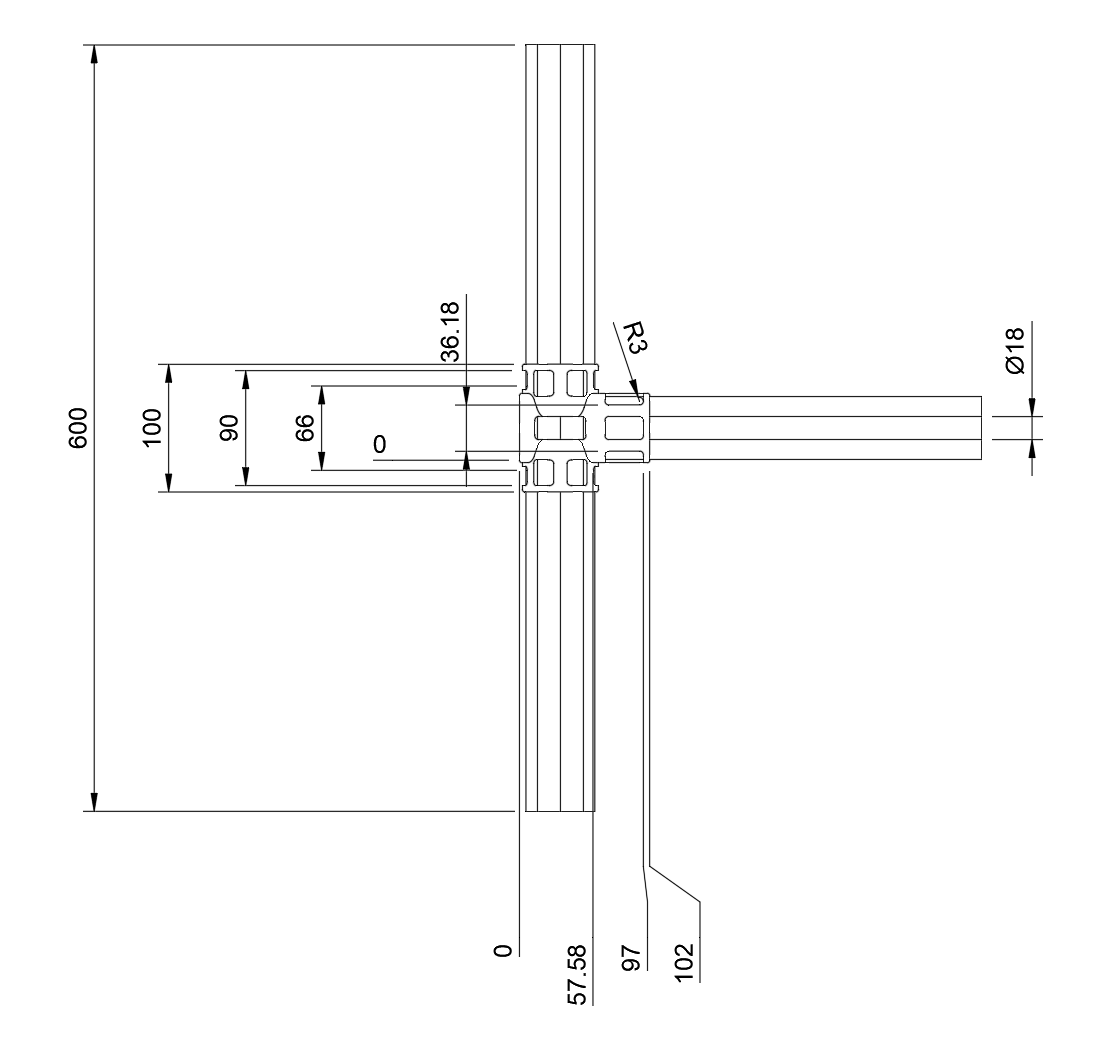
\includegraphics[width=0.75\textwidth]{figures/fig3_node_dimensions.png}
    \caption{T型节点连接件尺寸标注图}
    \label{fig:node_dimensions}
\end{figure}

图~\ref{fig:frame_assembly_dim}展示了骨架装配的整体尺寸标注，
骨架中心到旋翼保护圈中心的X方向距离为 338\,mm，Y方向距离为 333.45\,mm，
即旋翼的X方向轴距为 676\,mm，Y方向轴距为 666.9\,mm；
中心固定架相对骨架平面的抬高量为 76.53\,mm。

\begin{figure}[htbp]
    \centering
    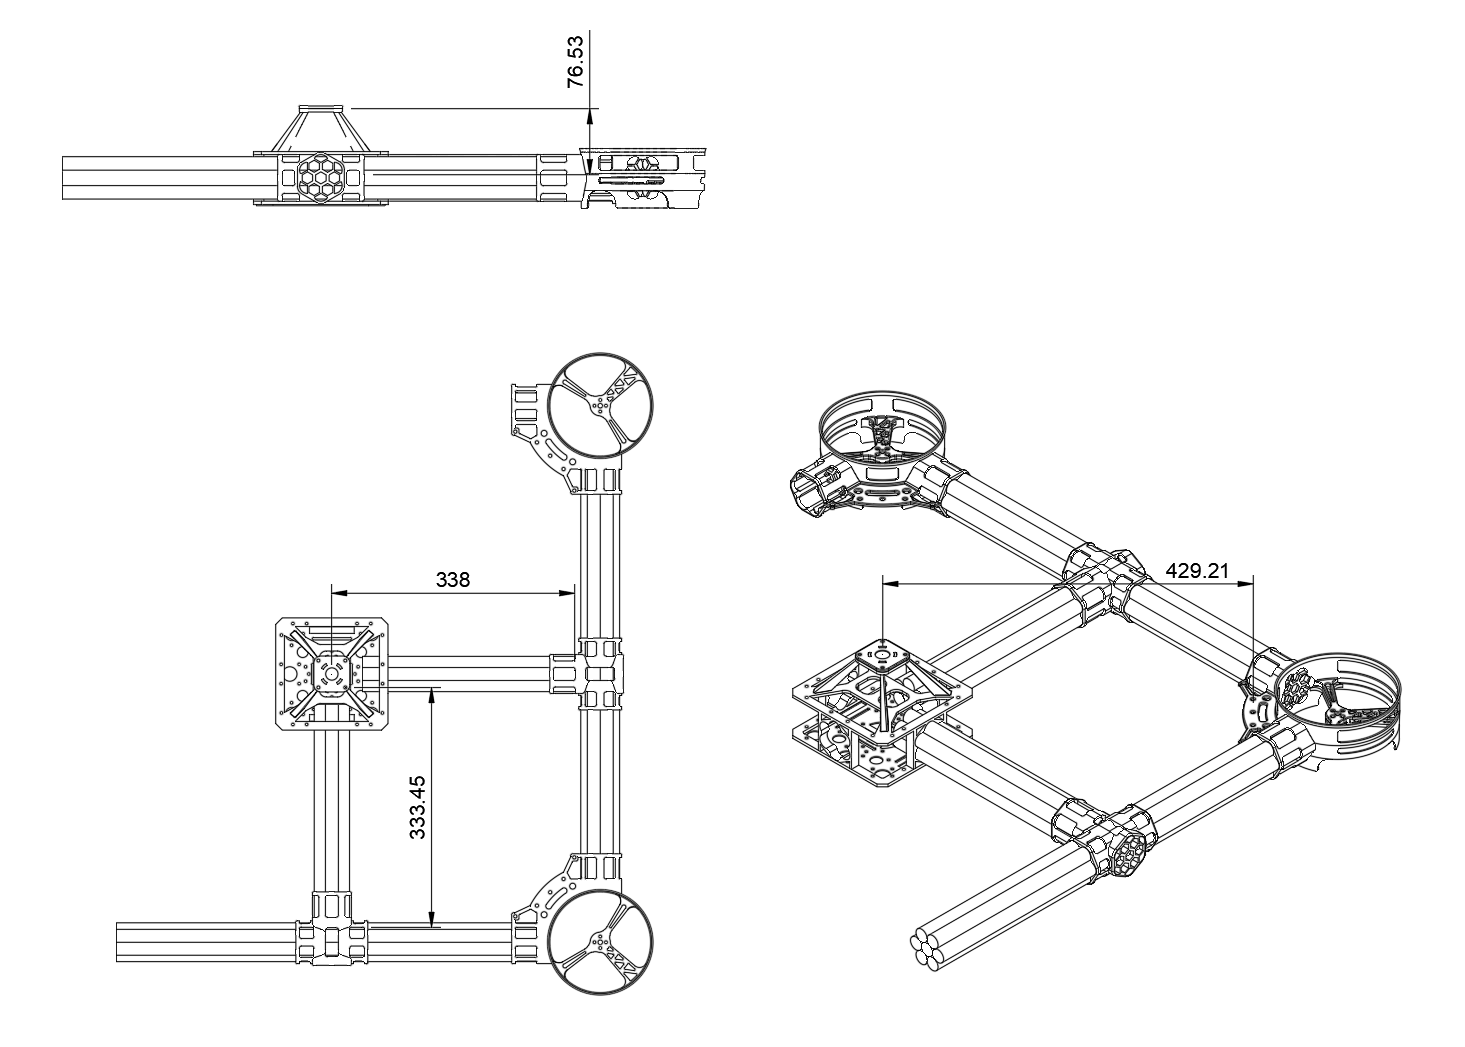
\includegraphics[width=0.85\textwidth]{figures/fig3_frame_assembly_dim.png}
    \caption{骨架装配尺寸标注图}
    \label{fig:frame_assembly_dim}
\end{figure}


% ----------------------------------------------------------
\section{TPU伞面设计}
\subsection{伞面材料选型}
伞面采用热塑性聚氨酯弹性体（TPU，Thermoplastic Polyurethane）薄膜材料。
选用TPU的主要依据如下：
\begin{itemize}
    \item \textbf{防水性能：}TPU薄膜具有优异的防水性能，在遮雨功能场景下表现可靠；
    \item \textbf{轻量化：}TPU薄膜面密度低，同等覆盖面积下重量远小于传统伞布；
    \item \textbf{柔性收纳：}TPU薄膜柔软可折叠，排气后可随气柱骨架一同压缩收纳；
    \item \textbf{耐候性：}TPU对紫外线、温度变化具有良好的适应性，适合户外长期使用。
\end{itemize}

\subsection{伞面几何设计与遮蔽面积}
TPU伞面铺设于骨架气柱的外侧并粘合固定，其水平投影形状为正方形。
伞面有效遮蔽边长取骨架外侧气柱外边缘到对边气柱外边缘的距离，
由CAD模型实测得该边长为 $L_{\text{shelter}} = 779.59$\,mm（约 77.96\,cm）。
伞面水平投影面积（正投影遮蔽面积）为：
\begin{equation}
    S = L_{\text{shelter}}^2 = (0.77959)^2 \approx 0.608\,\text{m}^2
    \label{eq:umbrella_area}
\end{equation}
相比之下，成人头肩部的遮蔽需求约为 $0.25\sim0.30$\,m$^2$。
本系统 0.608\,m$^2$ 的有效遮蔽面积在悬停精度良好的前提下可提供充裕的遮护裕量，
遮护面积冗余约 103\%\,$\sim$\,143\%。

\subsection{伞面倾角设计}
考虑到飞行雨伞在实际使用中需覆盖用户的头部及肩部区域，
伞面设计为具有一定向下倾斜角度的非水平结构，使伞面形成类似传统雨伞的拱形遮蔽形态，
同时有利于积水沿伞面边缘自然流下，避免积水在伞面中心造成附加质量。
伞面倾角由中心固定架的抬高量 $h$ 与水平投影距离 $d$ 共同决定。

根据图~\ref{fig:frame_assembly_dim}的侧视图尺寸标注，
中心固定架将伞面中心相对骨架平面抬高 $h = 76.53$\,mm。
水平投影距离取中心点到骨架边框中点的投影距离（即半轴距），
取X、Y方向的平均值 $d_{\text{avg}} = (338 + 333.45)/2 = 335.725$\,mm。
平均伞面倾角 $\alpha$ 计算如下：
\begin{equation}
    \alpha = \arctan\!\left(\frac{h}{d_{\text{avg}}}\right)
           = \arctan\!\left(\frac{76.53}{335.725}\right)
           \approx 12.8°
    \label{eq:tilt_angle}
\end{equation}
本系统伞面倾角约为 12.8°，
与传统雨伞伞面倾角（通常为 $10°\sim15°$）高度吻合，
能够完美满足积水引导与遮蔽形态的功能要求。


% ----------------------------------------------------------
% [图片占位 Fig.3.5] ★需要制作★
% 内容：伞面倾角设计侧视示意图
%   元素：水平骨架线、中心固定架（竖线）、伞面（从固定架顶端向四周倾斜的弧线）
%   标注：倾角15°、伞面覆盖直径72cm
%   用PowerPoint绘制即可，简洁清晰为主
% \begin{figure}[htbp]
%     \centering
%     \includegraphics[width=0.60\textwidth]{figures/fig3_5_umbrella_tilt.png}
%     \caption{伞面倾角设计示意图（侧视），倾角约15°}
%     \label{fig:umbrella_tilt}
% \end{figure}
% ----------------------------------------------------------


\section{充气展开系统}

\subsection{充气方式与设备选型}
本系统的充气骨架采用分腔充气设计：骨架气柱与伞面气柱分别独立充气，互不干扰。
充气操作通过骨架上预留的充气阀接口完成，使用标准气嘴与充气泵对接。

快递气柱的充气原理如图~\ref{fig:aircolumn_inflate} 所示。
气柱内部设有一条贯通全长的公共主气道，充气时气体由充气嘴进入主气道
并沿其横向流动；主气道沿途通过若干单向止回阀与各独立气室相连，
气体依次经由单向阀充入各气室，使气室膨胀成型。
气室内压达到平衡后，单向阀在内外压差作用下自动关闭，
各气室独立密封；多余气体经主气道末端排出。
这种结构还带来一个附带优点：即便个别气室破损，
其余气室仍可维持充气状态，不会导致整体骨架失效。

\begin{figure}[htbp]
    \centering
    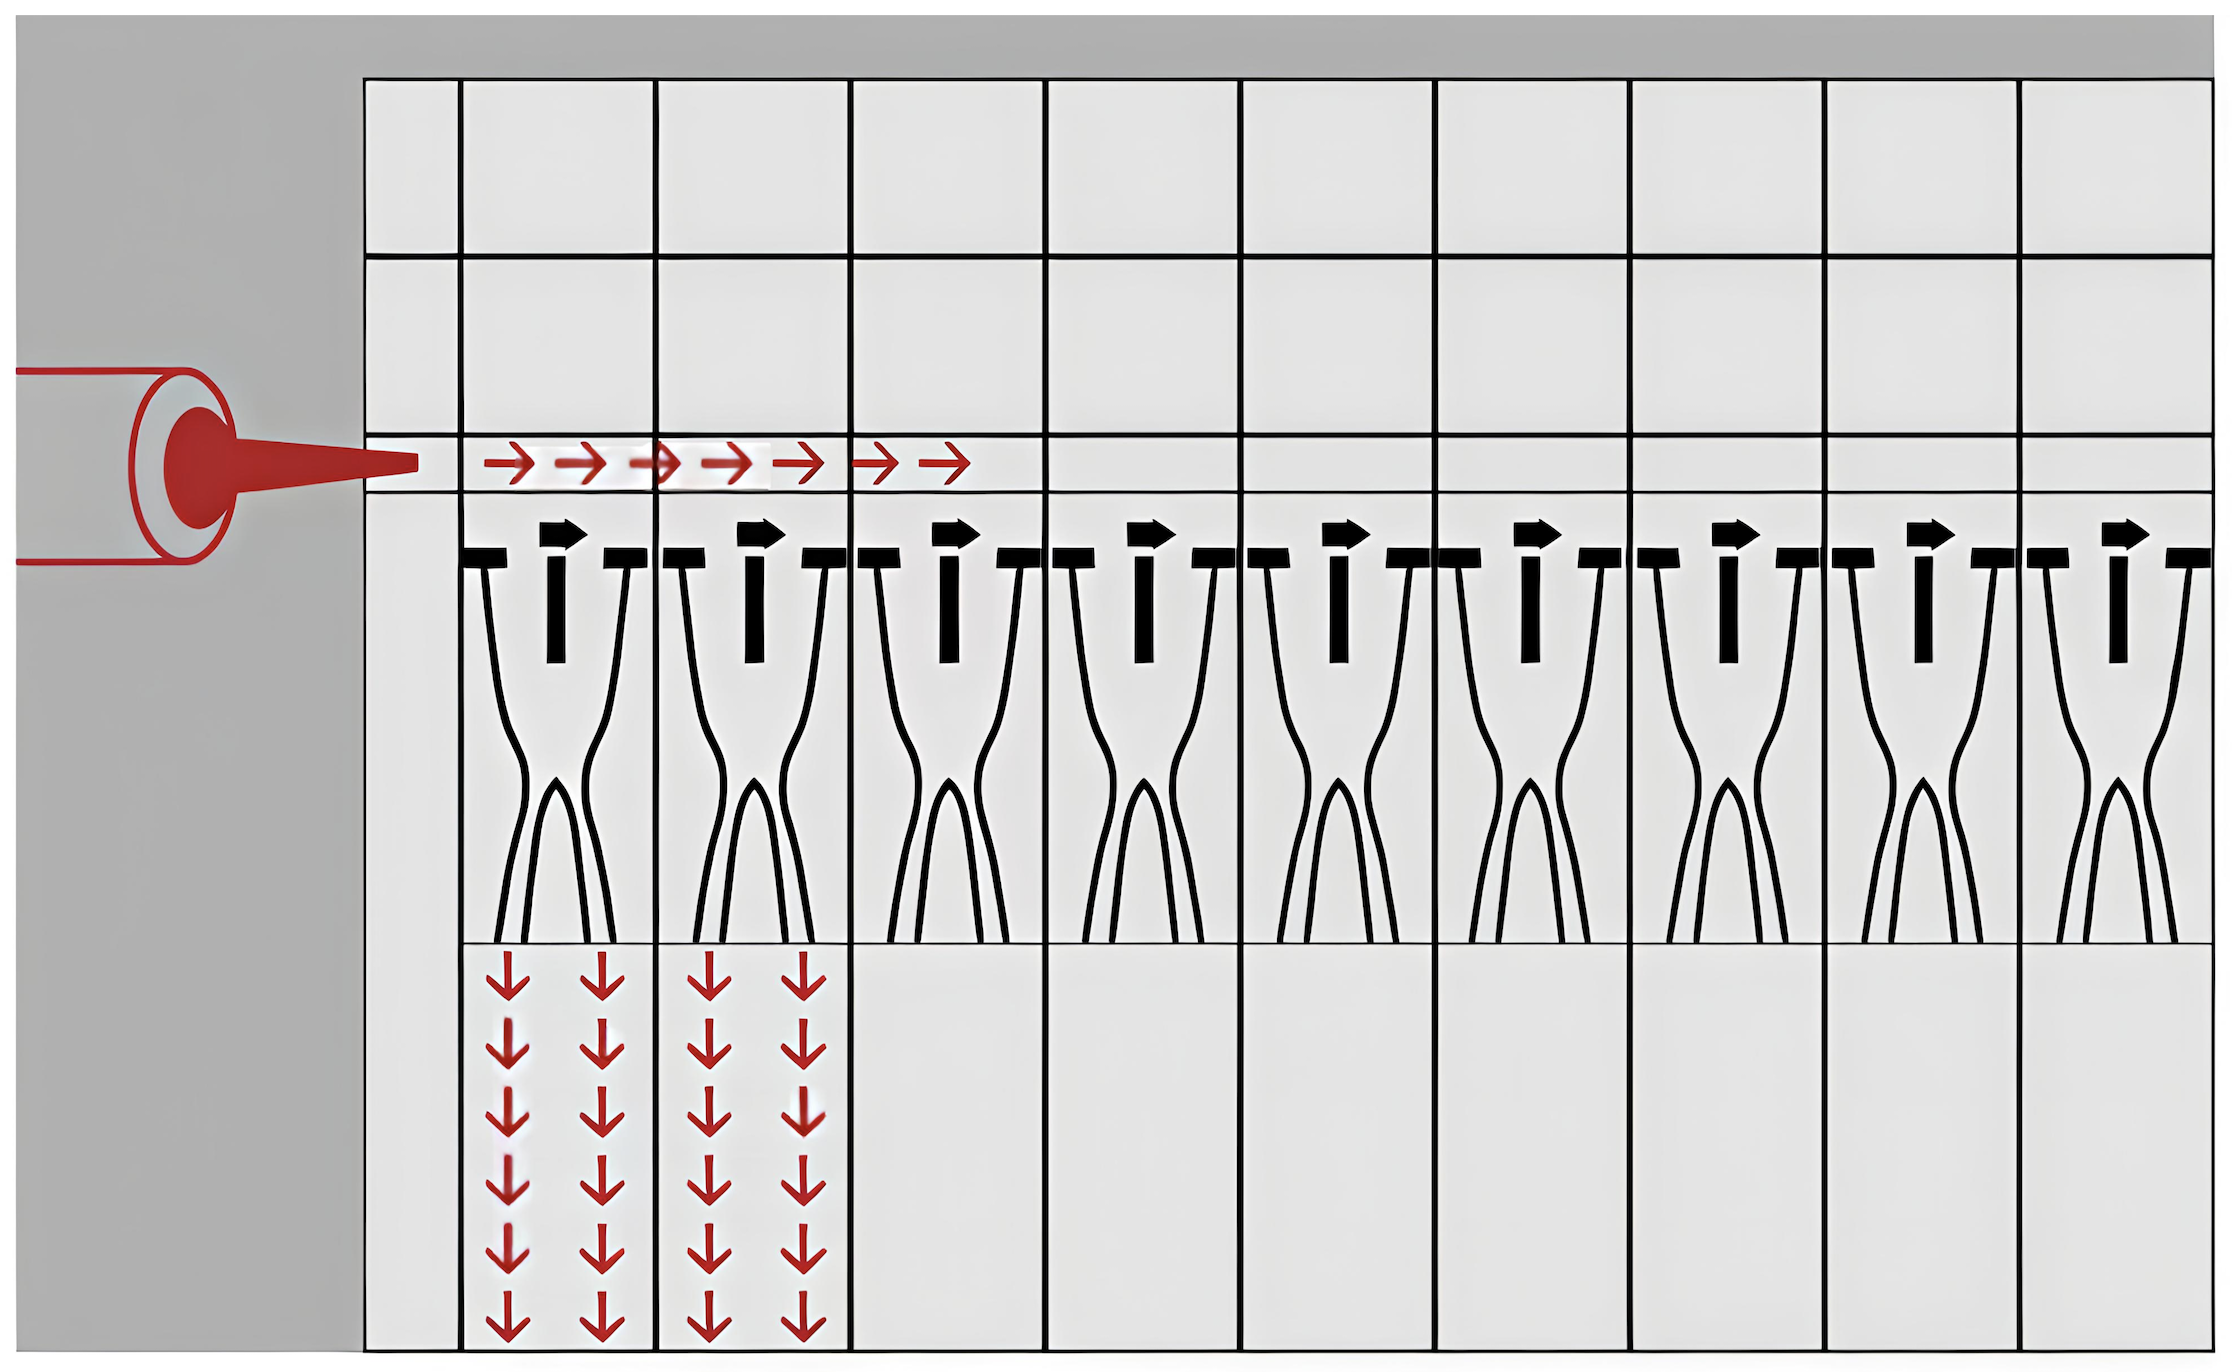
\includegraphics[width=0.65\textwidth]{figures/fig3_aircolumn_inflate.png}
    \caption{快递气柱充气工作原理示意图（单向阀自密封结构）}
    \label{fig:aircolumn_inflate}
\end{figure}

在样机验证阶段，采用车载 12\,V 微型充气泵进行充气操作，
充气时间约为 30$\sim$60\,s（视气柱总容积与泵的额定流量而定）。
充气完成后，充气阀自动密封，无需额外操作。

\subsection{气密性说明}
快递气柱采用PA复合薄膜热封工艺，气密性经过商业物流应用的充分验证。
在标准充气压力下，气柱可维持数小时至数天不发生明显漏气，
远超本系统单次使用的时间需求（约 5$\sim$10\,min）。
在实验阶段，气密保持时长测试结果详见第七章。



\section{本章小结}

本章完成了飞行雨伞充气骨架系统的设计。
系统以标准快递气柱为唯一结构承力件，配合 PLA 3D 打印节点
构成正方形模块化骨架，全程不使用刚性金属或碳纤维结构件。
骨架实物外框边长 870\,mm，对角旋翼轴距 1230\,mm，
TPU 伞面有效遮蔽面积约 0.608\,m$^2$。
充气展开采用车载微型充气泵，气密性满足单次使用需求。
上述结构参数将在第四章动力系统选型计算中作为输入条件使用。
